\subsubsection{Account Management}
\label{sec:account-management}

This functional area covers all use cases related to user accounts. Since the application's core functionality is expense management, user login is the only required action. The resulting use case diagram is presented in Figure \ref{fig:account-management-use-case-diagram}.

\begin{figure}[H]
    \centering
    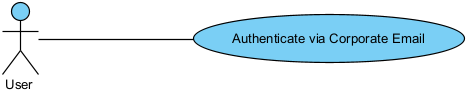
\includegraphics[width=0.6\textwidth]{Images/accountmanagement.png}
    \caption[Account management use case diagram]
    {Account management use case diagram. [Own creation]}
    \label{fig:account-management-use-case-diagram}
\end{figure}

\vspace{1cm}

\textbf{Use Case: Authenticate via Corporate Email}

\textbf{Primary Actor:} User

\textbf{Trigger:} The user attempts to access the application URL.

\textbf{Preconditions:} None.

\textbf{Postconditions:} The user is authenticated and redirected to the home page with role-specific access.

\vspace{0.5cm}

\textbf{Main Success Scenario:}

\begin{enumerate}  [leftmargin=0.75cm, noitemsep]
    \item The user navigates to the web application and initiates the login process.
    \item The system displays the login interface.
    \item The user enters their account credentials.
    \item The system authenticates the credentials successfully.
    \item The system verifies that the email belongs to the authorized corporate domain.
    \item The system assigns the corresponding role to the user and redirects them to the home page, displaying the available functionalities according to the user's assigned role.
\end{enumerate}

\vspace{0.3cm}

\textbf{Extensions:}

\begin{itemize} [label={}, leftmargin=0.75cm, noitemsep]
    \item \textbf{2a. Server Connection Error:}
    \begin{itemize} [label={}, leftmargin=0.75cm, noitemsep]
        \item 2a1. The system cannot connect to the server and cannot display the login interface.
    \end{itemize}

    \item \textbf{4a. Authentication Failed (Invalid Credentials):}
    \begin{itemize} [label={}, leftmargin=0.75cm, noitemsep]
        \item 4a1. The system displays an invalid credentials error message (``Invalid email'' or ``Invalid password'').
        \item 4a2. The user remains on the login page and returns to step 3 until valid credentials are provided.
    \end{itemize}

    \item \textbf{5a. Unauthorized Domain:}
    \begin{itemize}  [label={}, leftmargin=0.75cm, noitemsep]
        \item 5a1. The system detects that the authenticated account does not belong to the authorized corporate domain.
        \item 5a2. The system denies access and notifies the user.
    \end{itemize}
\end{itemize}


